\documentclass[a4paper,onecolumn]{article}
\usepackage[page,toc,titletoc,title]{appendix}
\usepackage{url}
\usepackage{subfigure}
\usepackage[sc]{mathpazo} % Use the Palatino font
\usepackage[T1]{fontenc} % Use 8-bit encoding that has 256 glyphs
\usepackage[utf8]{inputenc} % Use utf-8 as encoding
\linespread{1.05} % Line spacing - Palatino needs more space between lines
\usepackage{microtype} % Slightly tweak font spacing for aesthetics
\usepackage[spanish, activeacute]{babel}
 \decimalpoint
% \usepackage[hmarginratio=1:1,top=32mm,columnsep=20pt]{geometry} % Document marginshttps://www.overleaf.com/project/60211b96f72a79d4c7515e93
% \usepackage[hang, small,labelfont=bf,up,textfont=it,up]{caption} % Custom captions under/above floats in tables or figures
\usepackage{verbatim} % comentarios
\usepackage{listings}
\usepackage{xcolor}
\usepackage{float}
\lstset{
    inputencoding=utf8,
    language=SQL,
    frame=single,
    basicstyle=\ttfamily\small,
    keywordstyle=\color{blue}\bfseries,
    identifierstyle=\color{black},
    commentstyle=\color{gray}\itshape,
    stringstyle=\color{red},
    numbers=left,
    numberstyle=\tiny\color{gray},
    stepnumber=1,
    numbersep=10pt,
    showspaces=false,
    showstringspaces=false,
    breaklines=true,
    breakindent=0pt,
    breakatwhitespace=false,
    tabsize=2,
    captionpos=b
}
\setlength{\parskip}{0.8em}
\usepackage{natbib}
\usepackage{enumitem}
% \setlist[itemize]{noitemsep} % Make itemize lists more compact
% \usepackage{abstract} % Allows abstract customization
% \renewcommand{\abstractnamefont}{\normalfont\bfseries} % Set the "Abstract" text to bold
% \renewcommand{\abstracttextfont}{\normalfont\small\itshape} % Set the abstract itself to small italic text
\usepackage{titlesec}

\usepackage{fancyhdr} % Headers and footers
\pagestyle{fancy} % All pages have headers and footers
\fancyhead{}
\lhead{Hugo Gómez Sabucedo}
\rhead{Bases de datos SQL}

\renewcommand{\footrulewidth}{0.2pt}
\usepackage{titling} % Customizing the title section
\usepackage[breaklinks=true]{hyperref} % For hyperlinks in the PDF
%\usepackage{array}
%\newcolumntype{C}[1]{>{\centering\let\newline\\\arraybackslash\hspace{0pt}}m{#1}}
\usepackage{graphicx}
%\usepackage{lipsum} % NO NECESARIO LUEGO
%\usepackage{amsmath}
%\usepackage{wrapfig}
%\usepackage{multicol}
%\usepackage{bm}


\let\stdsection\section
\renewcommand\section{\newpage\stdsection}

%-------------------------------------------------------------------------------
%	TITLE SECTION
%-------------------------------------------------------------------------------

\setlength{\droptitle}{-4\baselineskip} % Move the title up



\title{\begin{center} \Huge Bases de datos NoSQL \end{center}} % Article title
\author{
    \textsc{\Huge Hugo Gómez Sabucedo} \\ % Your name
    \large \href{mailto:hugogomezsabucedo@gmail.com}{hugogomezsabucedo@gmail.com} \\ [2ex] % Your email address
    \Large \textbf{Máster Big Data, Data Science \& Inteligencia Artificial} \\
    \normalsize Curso 2024-2025 \\
    \large Universidad Complutense de Madrid
}
\date{} % Leave empty to omit a date

\begin{document}
% Print the title
\maketitle
%tableofcontents
\begin{sloppypar}

%-------------------------------------------------------------------------
%	DOCUMENT
%-------------------------------------------------------------------------

\section{Ejercicios} \label{ejericios}
A continuación se incluyen las capturas con las querys y los resultados de las ejecuciones de las consultas de los diferentes ejercicios, así como una breve 
explicación de las mismas (si es necesario). He incluido también el archivo \texttt{JavaScript} con todas las consultas al final del archivo y como adjunto.

\begin{enumerate} \setcounter{enumi}{-1}
    \item \textbf{Importación del fichero en una colección llamada movies}: se ha creado la colección movies dentro de la base de datos \textit{clases} e
    importado los datos usando la funcionalidad ''Add data'' de MongoDBCompass, importando los datos directamente desde el archivo JSON.
    \begin{center}
        \begin{figure}[h!]
            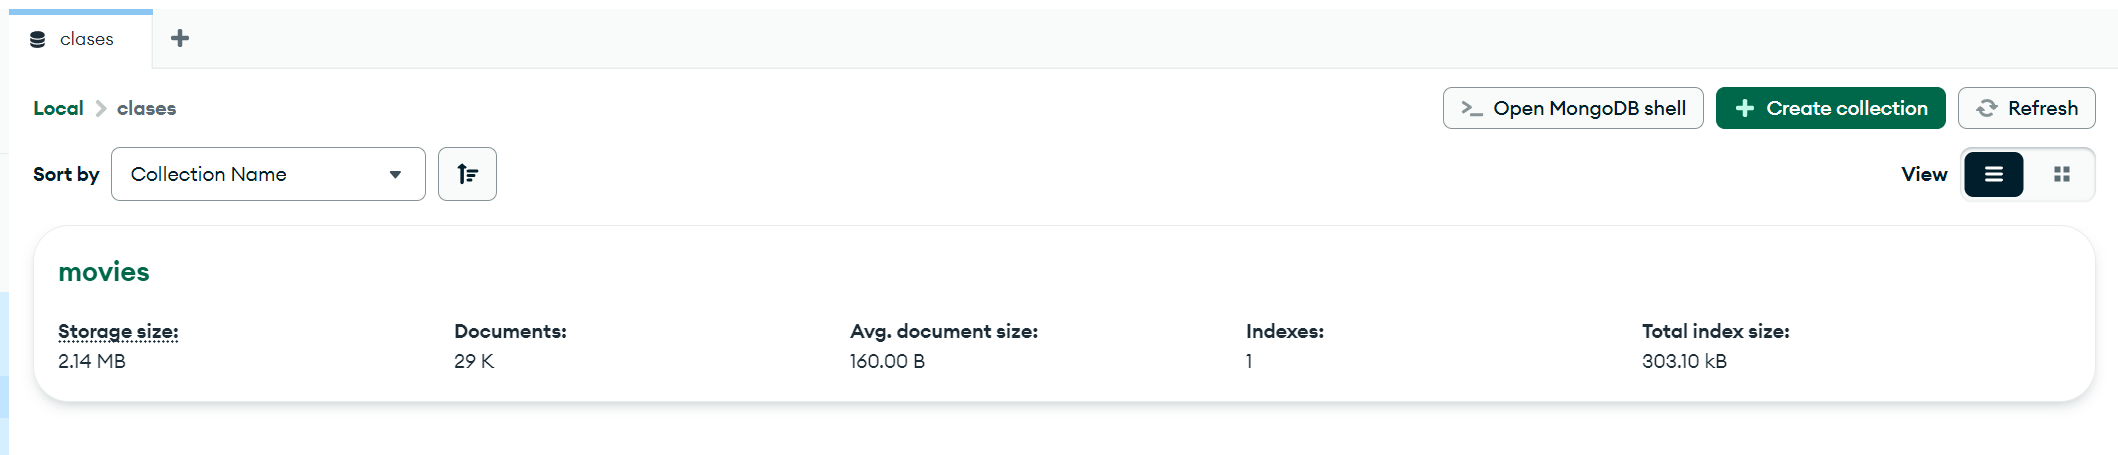
\includegraphics[width=\textwidth]{querys/0.png}
        \end{figure}
    \end{center}
    \item \textbf{Analizar con find la colección}.
    \begin{center}
        \begin{figure}[h!]
            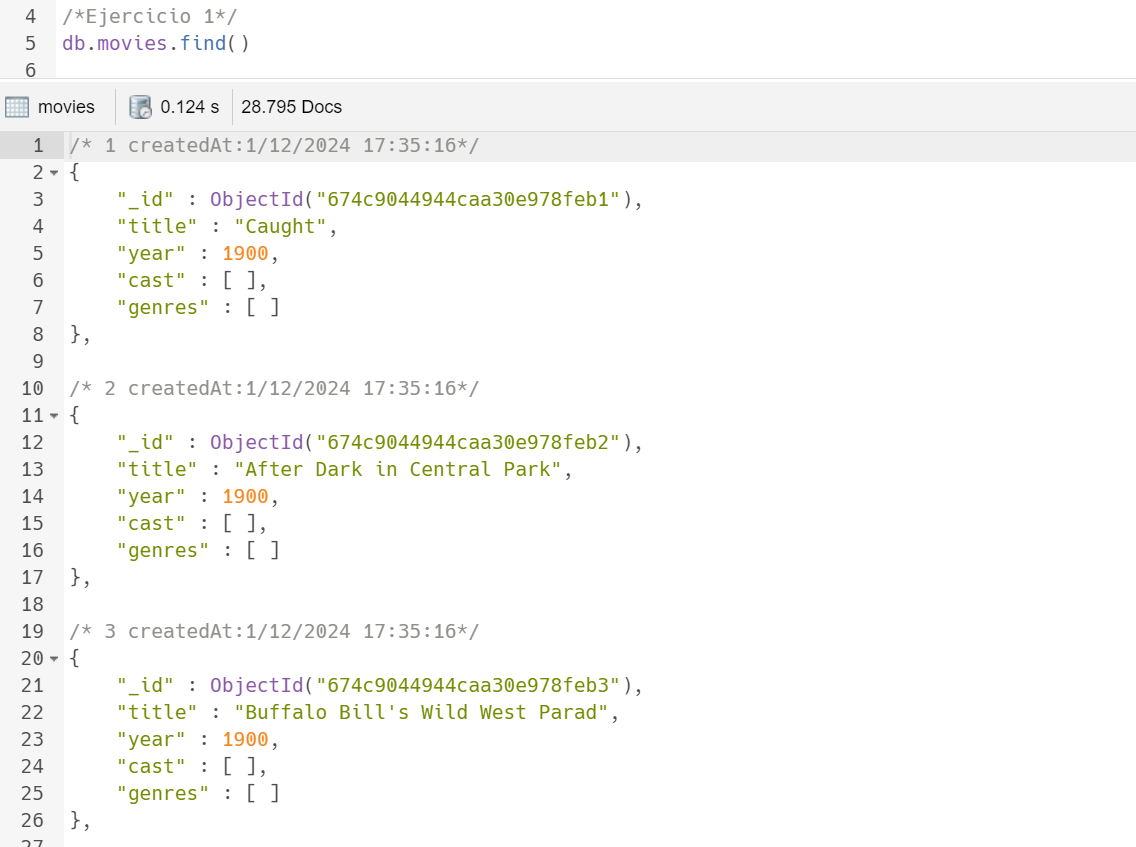
\includegraphics[width=\textwidth]{querys/1.png}
        \end{figure}
    \end{center}
    \item \textbf{Contar cuantos documentos (películas) tiene cargado}.
    \begin{center}
        \begin{figure}[H]
            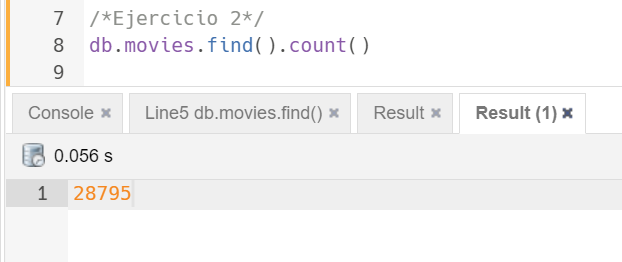
\includegraphics[width=\textwidth]{querys/2.png}
        \end{figure}
    \end{center}
    \item \textbf{Insertar una película}. Se crea una película \textit{test} para insertar.
    \begin{center}
        \begin{figure}[h!]
            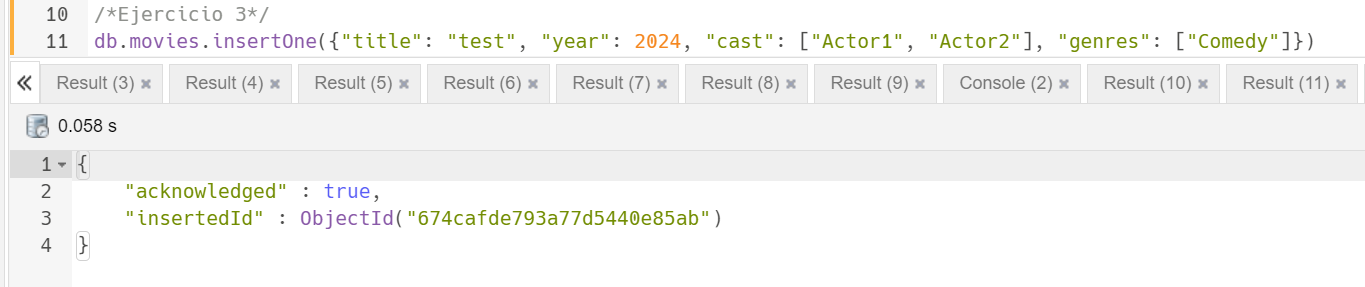
\includegraphics[width=\textwidth]{querys/3.png}
        \end{figure}
    \end{center}
    \item \textbf{Borrar la película insertada en el punto anterior}. Como la película se llama \textit{text} y es del año 2024 (más adelante se comprobará
    que no hay ninguna película de este año), se borra en base a esto. Borrar en base al id no es efectivo, ya que si se reejecuta la query este cambiará.
    \begin{center}
        \begin{figure}[h!]
            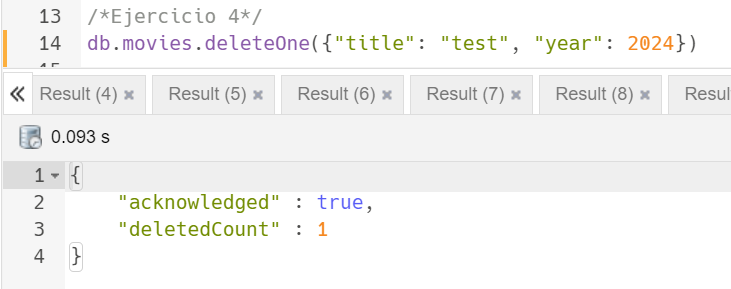
\includegraphics[width=\textwidth]{querys/4.png}
        \end{figure}
    \end{center}
    \item \textbf{Contar cuantas películas tienen actores que se llaman ''and''}.
    \begin{center}
        \begin{figure}[h!]
            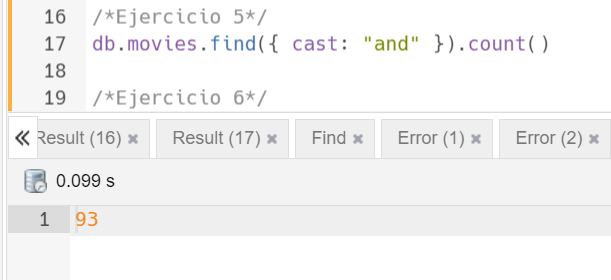
\includegraphics[width=\textwidth]{querys/5.png}
        \end{figure}
    \end{center}
    \item \textbf{Actualizar los documentos cuyo actor tenga el valor ''and'', sacando ese valor del array cast}.
    \begin{center}
        \begin{figure}[h!]
            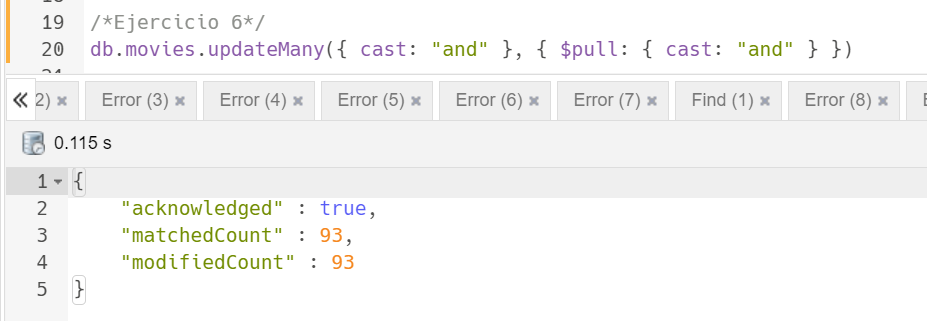
\includegraphics[width=\textwidth]{querys/6.png}
        \end{figure}
    \end{center}
    \item \textbf{Contar cuantos documentos tienen el array 'cast' vacío}.
    \begin{center}
        \begin{figure}[h!]
            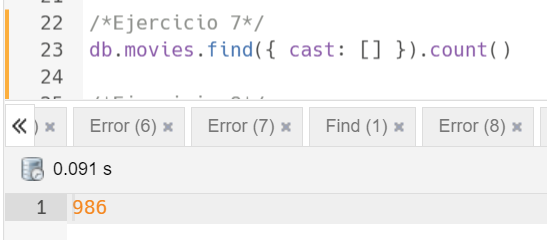
\includegraphics[width=\textwidth]{querys/7.png}
        \end{figure}
    \end{center}
    \item \textbf{Actualizar todos los documentos que tengan el array cast vacío, añadiendo un nuevo elemento con el valor Undefined}.
    \begin{center}
        \begin{figure}[h!]
            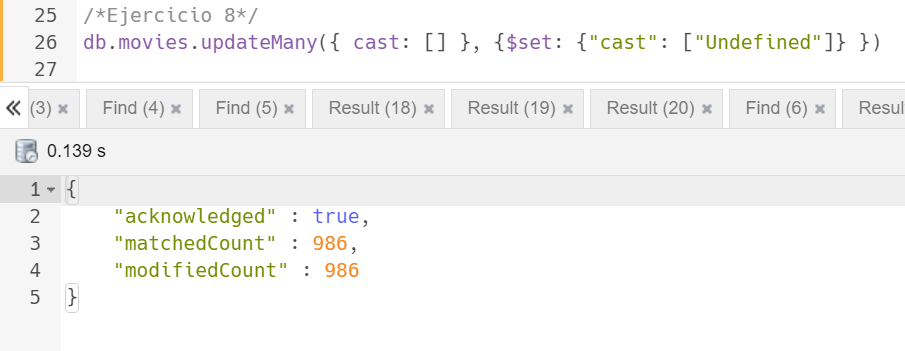
\includegraphics[width=\textwidth]{querys/8.png}
        \end{figure}
    \end{center}
    \item \textbf{Contar cuantos documentos tienen el array genres vacío}.
    \begin{center}
        \begin{figure}[h!]
            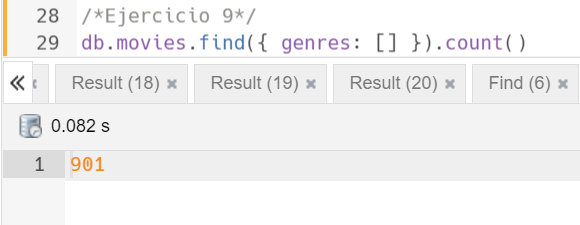
\includegraphics[width=\textwidth]{querys/9.png}
        \end{figure}
    \end{center}
    \item \textbf{Actualizar todos los documentos que tengan el array genres vacío, añadiendo un nuevo elemento con el valor Undefined}.
    \begin{center}
        \begin{figure}[h!]
            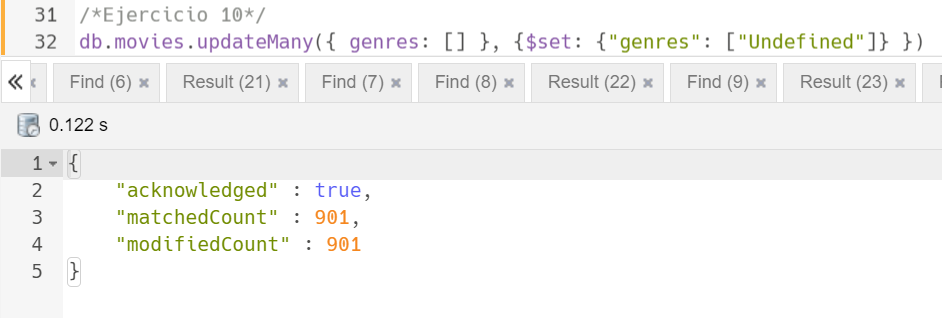
\includegraphics[width=\textwidth]{querys/10.png}
        \end{figure}
    \end{center}
    \item \textbf{Mostrar el año más reciente/actual que tenemos sobre todas las películas}.
    \begin{center}
        \begin{figure}[h!]
            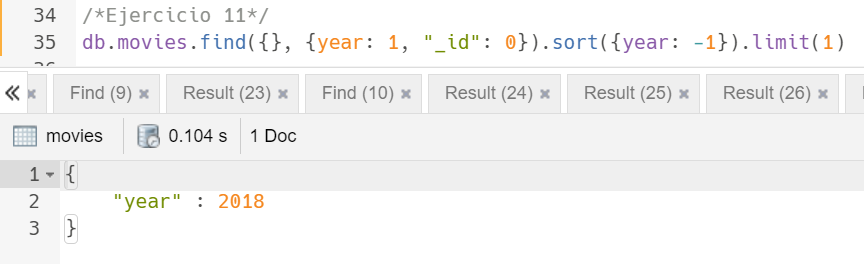
\includegraphics[width=\textwidth]{querys/11.png}
        \end{figure}
    \end{center}
    \item \textbf{Contar cuantas películas han salido en los últimos 20 años, desde el último año quee se tienen películas en la colección}.
    \begin{center}
        \begin{figure}[h!]
            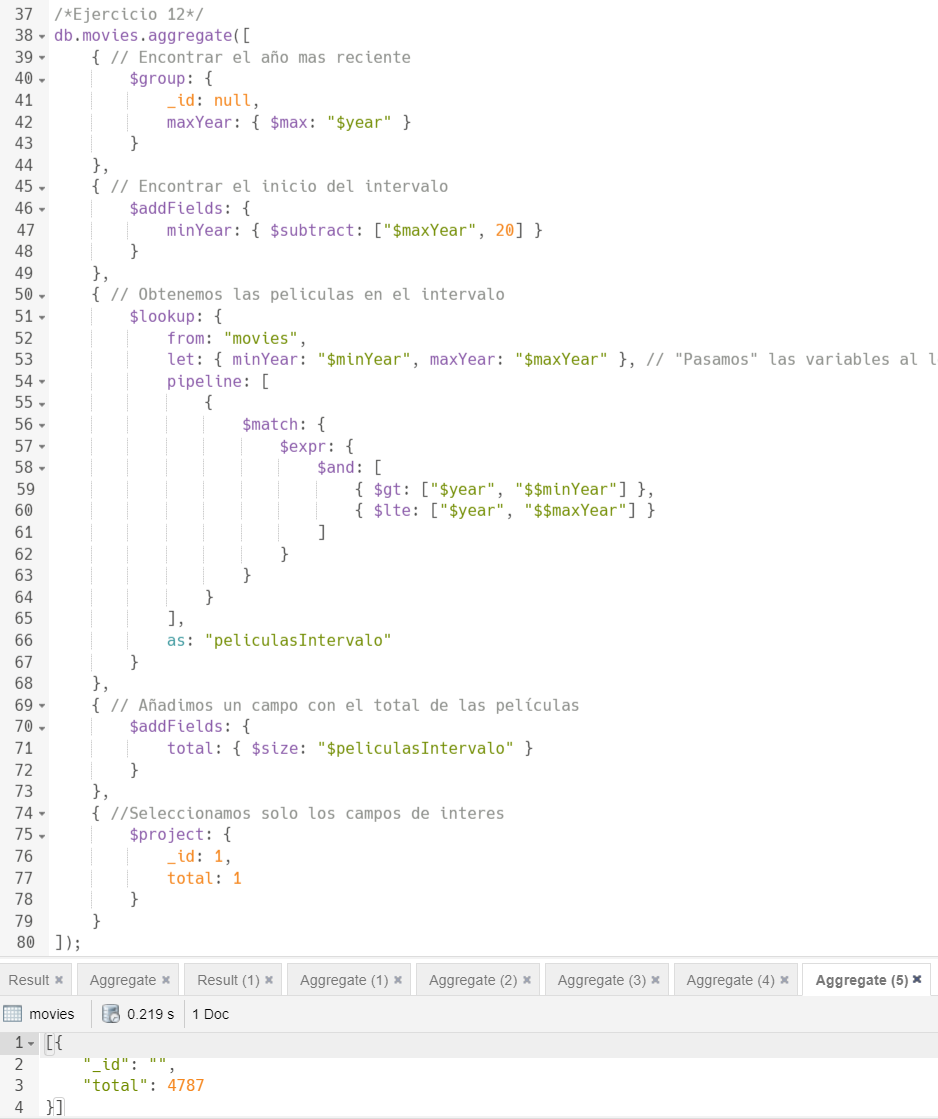
\includegraphics[width=\textwidth]{querys/12.png}
        \end{figure}
    \end{center}
    \item \textbf{Contar cuantas películas han salido en la década de los 60}.
    \begin{center}
        \begin{figure}[h!]
            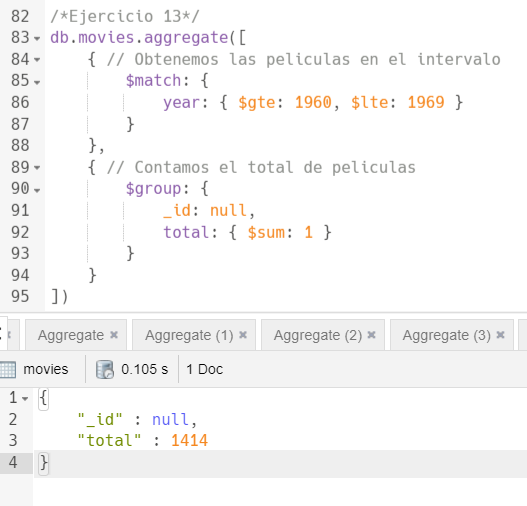
\includegraphics[width=\textwidth]{querys/13.png}
        \end{figure}
    \end{center}
    \item \textbf{Mostrar el año/años con más películas}.
    \begin{center}
        \begin{figure}[h!]
            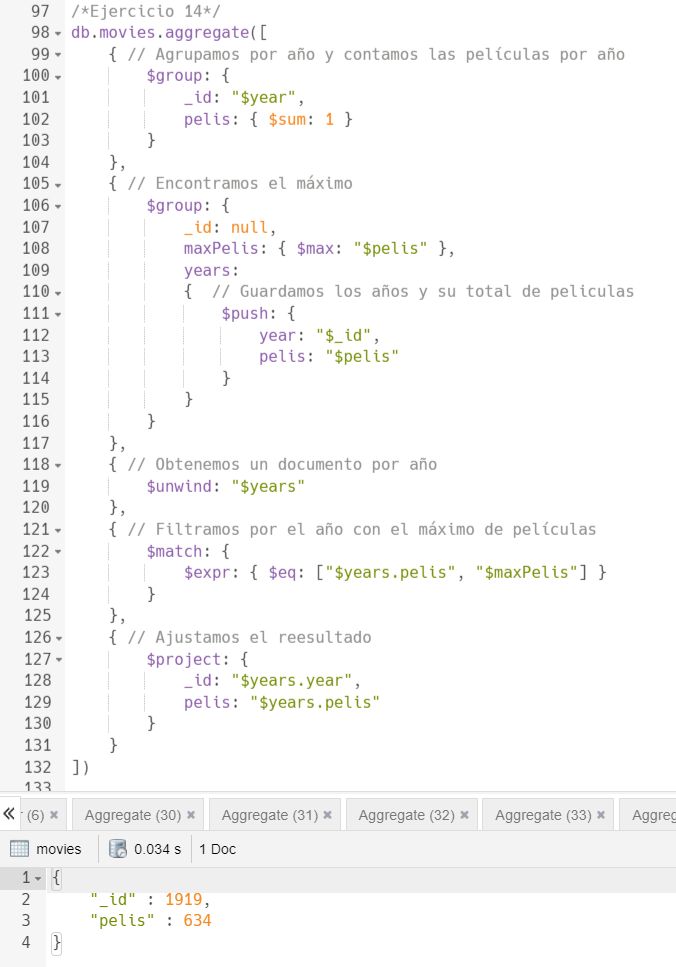
\includegraphics[width=\textwidth]{querys/14.png}
        \end{figure}
    \end{center}
    \item \textbf{Mostrar el año/años con menos películas}.
    \begin{center}
        \begin{figure}[h!]
            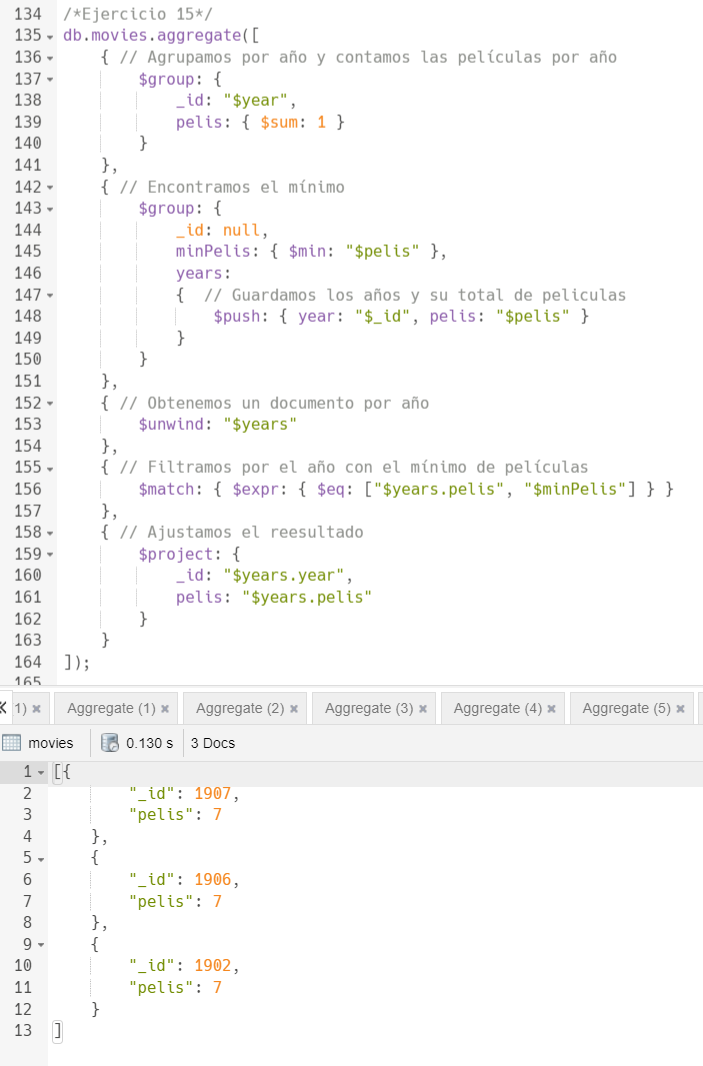
\includegraphics[width=\textwidth]{querys/15.png}
        \end{figure}
    \end{center}
    \item \textbf{Guardar en una nueva colección llamada ''actors'', haciendo \$unwind por actor. Contar cuantos elementos existen en la nueva colección}.
    \begin{center}
        \begin{figure}[h!]
            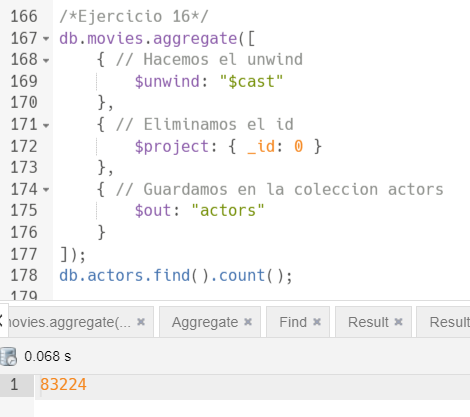
\includegraphics[width=\textwidth]{querys/16.png}
        \end{figure}
    \end{center}
    \item \textbf{Sobre \underline{actors}, mostrar la lista con los 5 actores que han participado en más películas, mostrando el número de películas en las que ha participado}.
    \begin{center}
        \begin{figure}[h!]
            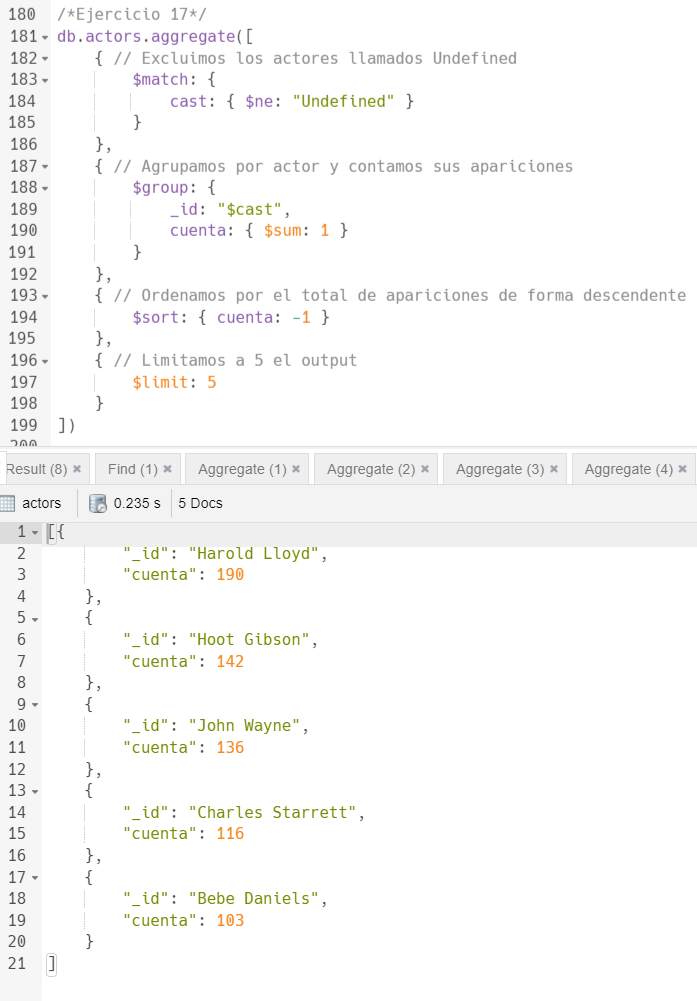
\includegraphics[width=\textwidth]{querys/17.png}
        \end{figure}
    \end{center}
    \item \textbf{Sobre \underline{actors}, agrupar por película y año, mostrando las 5 en las que más actores hayan participado, mostrando el número total de actores}.
    \begin{center}
        \begin{figure}[h!]
            %\includegraphics[width=\textwidth]{querys/.png}
        \end{figure}
    \end{center}
    \item \textbf{Sobre \underline{actors}, mostrar los 5 actores cuya carrera haya sido la más larga, mostrando cuando comenzó, cuando finalizó y cuántos años ha trabajado}.
    \begin{center}
        \begin{figure}[h!]
            %\includegraphics[width=\textwidth]{querys/.png}
        \end{figure}
    \end{center}
    \item \textbf{Sobre \underline{actors}, guardar en una nueva colección llamada ''genres'' realizando la fase \$unwind por genres. Contar cuantos elementos existen en al nueva colección}.
    \begin{center}
        \begin{figure}[h!]
            %\includegraphics[width=\textwidth]{querys/.png}
        \end{figure}
    \end{center}
    \item \textbf{Sobre \underline{genres}, mostrar los 5 documentos agrupados por Año y Género que más número de películas diferentes tienen, mostrando el total de películas}.
    \begin{center}
        \begin{figure}[h!]
            %\includegraphics[width=\textwidth]{querys/.png}
        \end{figure}
    \end{center}
    \item \textbf{Sobre \underline{genres}, mostrar los 5 actores y lo géneros en los que han participado con más número de géneros diferentes, mostrando el número de géneros}.
    \begin{center}
        \begin{figure}[h!]
            %\includegraphics[width=\textwidth]{querys/.png}
        \end{figure}
    \end{center}
    \item \textbf{Sobre \underline{genres}, mostrar las 5 películas y su año, en los que más géneros diferentes han sido catalogados, mostrando esos géneros y el número}.
    \begin{center}
        \begin{figure}[h!]
            %\includegraphics[width=\textwidth]{querys/.png}
        \end{figure}
    \end{center}
    \item \textbf{Ejercicio libre. Mostrar la películas con el reparto más grande, es decir, con el mayor número de actores. Mostrar la película, el año, los actores y el tamaño del cast}.
    \begin{center}
        \begin{figure}[h!]
            %\includegraphics[width=\textwidth]{querys/.png}
        \end{figure}
    \end{center}
    \item \textbf{Ejercicio libre. Sobre \underline{actors}, mostrar el actor más popular en cada género (es decir, el que más veces ha actuado)}. 
    \begin{center}
        \begin{figure}[h!]
            %\includegraphics[width=\textwidth]{querys/.png}
        \end{figure}
    \end{center}
    \item \textbf{Ejercicio libre. Sobre \underline{genres}, mostrar el génenro más popular en cada década, mostrando su nombre y el total de películas}. 
    \begin{center}
        \begin{figure}[h!]
            %\includegraphics[width=\textwidth]{querys/.png}
        \end{figure}
    \end{center}
\end{enumerate}

\end{sloppypar}

\section{Querys de los ejercicios}
\lstinputlisting{querys/querys_noSQL.js}
\end{document}
